\documentclass{beamer}

\mode<presentation> {

% The Beamer class comes with a number of default slide themes
% which change the colors and layouts of slides. Below this is a list
% of all the themes, uncomment each in turn to see what they look like.

%\usetheme{default}
%\usetheme{AnnArbor}
%\usetheme{Antibes}
%\usetheme{Bergen}
%\usetheme{Berkeley}
%\usetheme{Berlin}
%\usetheme{Boadilla}
%\usetheme{CambridgeUS}
%\usetheme{Copenhagen}
%\usetheme{Darmstadt}
%\usetheme{Dresden}
\usetheme{Frankfurt}
%\usetheme{Goettingen}
%\usetheme{Hannover}
%\usetheme{Ilmenau}
%\usetheme{JuanLesPins}
%\usetheme{Luebeck}
%\usetheme{Madrid}
%\usetheme{Malmoe}
%\usetheme{Marburg}
%\usetheme{Montpellier}
%\usetheme{PaloAlto}
%\usetheme{Pittsburgh}
%\usetheme{Rochester}
%\usetheme{Singapore}
%\usetheme{Szeged}
%\usetheme{Warsaw}

% As well as themes, the Beamer class has a number of color themes
% for any slide theme. Uncomment each of these in turn to see how it
% changes the colors of your current slide theme.

%\usecolortheme{albatross}
%\usecolortheme{beaver}
%\usecolortheme{beetle}
\usecolortheme{crane}
%\usecolortheme{dolphin}
%\usecolortheme{dove}
%\usecolortheme{fly}
%\usecolortheme{lily}
%\usecolortheme{orchid}
%\usecolortheme{rose}
%\usecolortheme{seagull}
%\usecolortheme{seahorse}
%\usecolortheme{whale}
%\usecolortheme{wolverine}

%\setbeamertemplate{footline} % To remove the footer line in all slides uncomment this line
%\setbeamertemplate{footline}[page number] % To replace the footer line in all slides with a simple slide count uncomment this line

%\setbeamertemplate{navigation symbols}{} % To remove the navigation symbols from the bottom of all slides uncomment this line
}

\usepackage{extpfeil}
\usepackage{extarrows} %Allows long equation signs
\usepackage{graphicx} % Allows including images
\usepackage{booktabs} % Allows the use of \toprule, \midrule and \bottomrule in tables
\usepackage{physics}
\usepackage{tikz}
\usepackage{cite}
%花体字母
\usepackage{amsthm,amsmath,amssymb}
\usepackage{mathrsfs}
\usepackage{dutchcal}
\usepackage{circuitikz}

%----------------------------------------------------------------------------------------
%	TITLE PAGE
%----------------------------------------------------------------------------------------

\title[VP260 RC]{VP260 Recitation Class 2} % The short title appears at the bottom of every slide, the full title is only on the title page

\author{Yanjun Chen} % Your name
\institute[UM-SJTU JI] % Your institution as it will appear on the bottom of every slide, may be shorthand to save space
{
    University of Michigan - Shanghai Jiao Tong University Joint Institute\\% Your institution for the title page
\medskip
}
\date{\today} % Date, can be changed to a custom date

\begin{document}

\begin{frame}
    \titlepage % Print the title page as the first slide
\end{frame}

%----------------------------------------------------------------------------------------
%	 SECTION 1
%----------------------------------------------------------------------------------------

\begin{frame}{Homework 1}
    \begin{itemize}
        \item Remember to indicate the direction of any vector!
    \end{itemize}

    \begin{block}{Approximation method}
        \begin{itemize}
            \item Taylor series;
            \item Bernoulli's inequality.
            
            If $x > -1$, then
            \begin{equation}
                (1 + x)^r \geq 1 + rx
            \end{equation}
            for $r \geq 1$ or $r \leq 0$.
        \end{itemize}
    \end{block}

\end{frame}


\section{Fundamental Concepts} % Section title slide, unnumbered

%------------------------------------------------

\begin{frame}{The Helmholtz's Theorem}
    \begin{block}{The Helmholtz's Theorem (not rigorous)}
        Let $\va{F}(\va{r})$  be a continuous vector field, which is continuously partial differentiable, then $\va{F}(\va{r})$ can be uniquely decomposed into two components,
        \begin{equation}
            \va{F} (\va{r}) = -\grad{\varphi(\va{r})} + \curl{\va{A}(\va{r})}.
        \end{equation}
    \end{block}

    \begin{itemize}
        \item The first component $\varphi(\va{r})$ is called scalar potential and the second component $\va{A} (\va{r})$ is called vector potential.
        \item Why?
        \begin{equation}
            \div{\va{F}} = \div(-\grad{\varphi} + \curl{\va{A}}) = -\laplacian{\varphi}
        \end{equation}
        \begin{equation}
            \curl{\va{F}} = \curl(-\grad{\varphi} + \curl{\va{A}}) = \curl(\curl{\va{A}})
        \end{equation}
    \end{itemize}

\end{frame}

\begin{frame}{Scalar Potential and Conservative Vector Field}	
    \begin{columns}
        \column{0.7\textwidth}
        \begin{block}{Conservative vector field}
            For a conservative vector field $\va{F}(\va{r})$, the following conditions are equivalent,
            \begin{itemize}
                \item Line integral $\int_{\vb{a}}^{\va{b}} \va{F} \vdot \dd{\vb{l}}$ is path independent;
                \item $\oint \va{F} \vdot \dd{\vb{l}} = 0$ for any closed loop;
                \item $\curl{\va{F}} = 0$ everywhere;
                \item Exists a function $\varphi$, s.t. $\va{F} = -\grad{\varphi}$.
            \end{itemize}
        \end{block}

        \begin{itemize}
            \item This is valid in simple-connected region.
        \end{itemize}


        \column{0.3\textwidth}
        \begin{figure}[H]
            \centering
            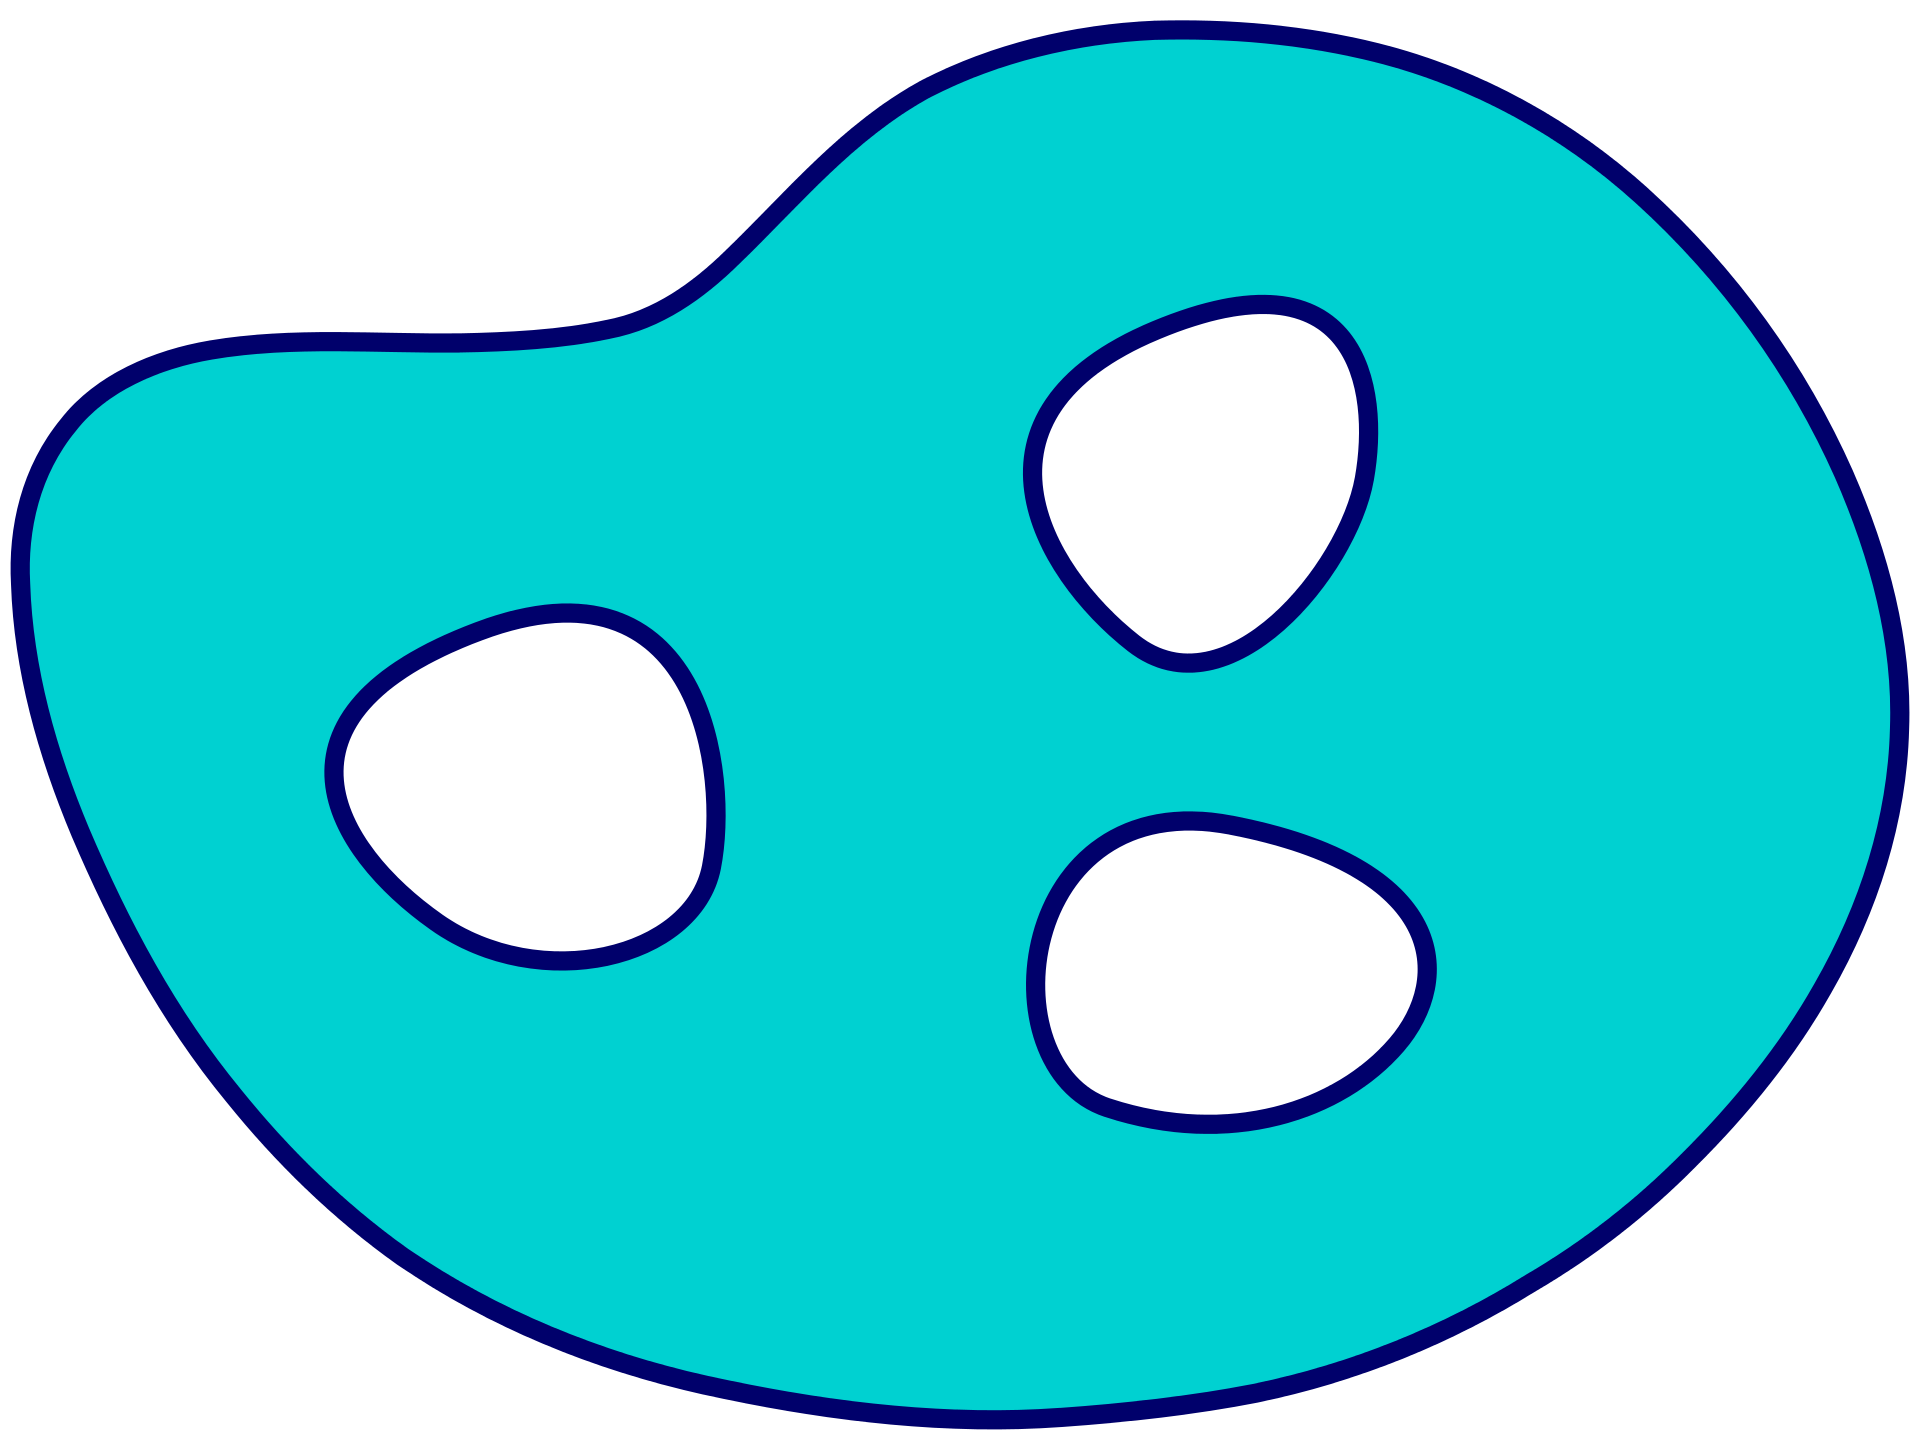
\includegraphics[height=1cm]{Images/sconnect.png}
        \end{figure}
        \vspace{5.5em}
        
    \end{columns}
\end{frame}


\begin{frame}{Conservative Vector Field}
    \begin{block}{How to argue that central vector field is conservative?}
        \begin{equation}
            \grad_{(r,\theta,\phi)} \times f(r)\vu*{r} = \frac{\vu*{e}_{\theta}}{r}\frac{1}{\sin \theta} \frac{\partial f(r)}{\partial \varphi}
            -\frac{\vu*{e}_{\varphi}}{r}\frac{\partial f(r)}{\partial \theta}
        \end{equation}
        \begin{equation*}
            \Rightarrow \grad_{(r,\theta,\phi)} \times f(r)\vu*{r} = \va*{0}
        \end{equation*}
    \end{block}

    % \begin{block}{\bf For any central force:}
    %     \begin{equation*}
    %         U_A - U_B = \int_{\abs*{\va*{r_A}}}^{\abs*{\va*{r_B}}} f(r)\vu*{r} \cdot \dd{\va*{r}}
    %     \end{equation*}
    % \end{block}

\end{frame}


\begin{frame}{Electric Potential}
    We can prove that electric field is conservative.
    \begin{equation}
        \curl{\va{E}} = 0.
    \end{equation}

    \begin{block}{Electric potential}
        \begin{equation}
            V(\va{r}) = -\int_O^{\va{r}} \va{E} \vdot \dd{\va{l}}
        \end{equation}

        \begin{itemize}
            \item Here, point O is zero reference. We use infinity as reference point usually.
            \item Unit: [V]olt
        \end{itemize}
		% \begin{equation}
		% 	U = \frac{1}{4\pi\epsilon_0}\frac{qq_0}{\abs*{\va*{\mathbcal{r}}}}
		% \end{equation}	
    \end{block}
\end{frame}


\begin{frame}{Potential energy}
    Move a test charge $q$ from point $\va{a}$ to $\va{b}$, the minimum work is,
    \begin{equation}
        W = \int_{\vb{a}}^{\vb{b}} \va{F} \vdot \dd{\va{l}} = -q \int_{\vb{a}}^{\vb{b}} \va{E} \vdot \dd{\va{l}} = q \cdot (V(\va{a}) - V(\va{b}))
    \end{equation}

    \begin{block}{Potential energy}
        \begin{equation}
            U(\va{r}) = q \cdot V(\va{r})
        \end{equation}
    \end{block}

    \begin{itemize}
        \item The minimum work for moving a test charge $q$ from point $\va{a}$ to $\va{b}$ is $U(\va{a}) - U(\va{b})$.
    \end{itemize}

    % \vspace{.5em}
	% \begin{beamerboxesrounded}[shadow=true]{\bf Configuration Potential Energy}
    %         \begin{equation}
    %             U_0 = \frac{q_0}{4\pi\epsilon_0}\sum_{i=1}^n\frac{q_i}{\abs*{\va*{\mathbcal{r_{0i}}}}}
    %         \end{equation}
    %         \begin{equation}
    %             U_{conf} = \frac{1}{4\pi\epsilon_0}\sum_{i,j=1;i<j}^n\frac{q_iq_j}{\abs*{\va*{\mathbcal{r_{ij}}}}}
    %             = \frac{1}{8\pi\epsilon_0}\sum_{i,j=1;i \neq j}^n \frac{q_iq_j}{\abs*{\va*{\mathbcal{r_{ij}}}}}
    %             = \frac{1}{2}\sum_{i=1}^n q_i V(\va*{r_i})
    %         \end{equation}
    % \end{beamerboxesrounded}
\end{frame}

\begin{frame}{Point Charge and Electric Potential}
    For a point charge $q$ in origin, we choose infinity as zero reference, then,
    \begin{equation}
        V(r) = -\int_{\infty}^{\va{r}} \va{E} \vdot \dd{\va{l}} = \eval{\frac{1}{4 \pi \epsilon_0} \frac{q}{r'}}_{\infty}^r = \frac{1}{4 \pi \epsilon_0} \frac{q}{r}.
    \end{equation}

    For a collection of charges $q_1, q_2, \cdots, q_n$, the potential will be,

    \begin{equation}
        V(\va{r}) = \frac{1}{4 \pi \epsilon_0} \sum_{i = 0}^{n} \frac{q_i}{\abs{\mathbcal{r}_i}},
    \end{equation}
    where the $\mathbcal{r}_i$ is the distance between $\va{r}$ and i-th charge.

    % \begin{beamerboxesrounded}[shadow=true]{\bf Formulas}
    %     \begin{equation}
    %         V = \frac{U}{q_0} = \frac{1}{4\pi\epsilon_0}\frac{q}{\abs*{\va*{\mathbcal{r}}}}
    %     \end{equation}
    %     \begin{equation}
    %         V(\va*{r}) - V(\infty) = \int_{\va*{r}}^{\infty} \va*{E}(\va*{r'}) \cdot \dd{\va*{r'}}
    %     \end{equation}
    % \end{beamerboxesrounded}
    % \vspace{.5em}
\end{frame}

\begin{frame}{Continuous Charge Distribution and Electric Potential}
    From the formula of point charge, it is not hard to get the formula for continuous distribution:

    \begin{equation}
        V(\va{r}) = \frac{1}{4 \pi \epsilon_0} \int \frac{\rho(\va{r'})}{\mathbcal{r}} \dd{\tau},
    \end{equation}
    where $\va{\mathbcal{r}} = \va{r'} - \va{r}$.

    % TODO
    % \begin{itemize}
    %     \item How to find the electric potential distribution along the central axis of a uniformly charged ring?
    %     \item How to find the electric potential distribution inside and outside a uniformly charged conducting ball?
    % \end{itemize}
\end{frame}

\begin{frame}{Configuration Energy}
    Discrete distribution,
    \begin{equation}
        U_{conf} = \frac{1}{8 \pi \epsilon_0} \sum_{i} \sum_{j, i \neq j} \frac{q_i q_j}{r_{ij}} = \frac{1}{2} \sum_{i} q_i V(\va{r_i}).
    \end{equation}

    Continuous distribution,
    \begin{equation}
        U_{conf} = \frac{1}{2} \int_{\Omega} \rho V \dd{\tau} = \frac{\epsilon_0}{2} \left( \oint_{\Sigma} V \va{E} \vdot \dd{\va{A}} + \int_{\Omega} E^2 \dd{\tau} \right).
    \end{equation}

    For the whole space,
    \begin{equation}
        U_{conf} = \frac{\epsilon_0}{2} \int_{\mathbb{R}^3} E^2 \dd{\tau}.
    \end{equation}
\end{frame}

\begin{frame}{Conductor}
    \begin{itemize}
        \item Electric field lines is perpendicular to equipotential surfaces;
        \item The surface of a conductor is equipotential (electrostatic).
    \end{itemize}
    \vspace{1em}
    \begin{beamerboxesrounded}[shadow=true]{Properties of Conductors}
        \begin{itemize}
            \item $\va{E} = 0$ \textbf{everywhere} inside a conductor;
            \item Any excess charge placed on a conductor resides entirely on its surface;
            \item Any conductor is equipotential.
        \end{itemize}
    \end{beamerboxesrounded}
\end{frame}


\begin{frame}{Poisson's Equation}
    \begin{block}{Recall: (Gauss' Law)}
        \begin{equation}
            \div{\va{E}} = \frac{\rho}{\epsilon_0}
        \end{equation}  
        \text{Since $\va{E} = -\grad{V}$, then we have:}
        \begin{equation}
            \div(-\grad{V}) = -\laplacian{V} = \frac{\rho}{\epsilon_0}
        \end{equation}
    \end{block}

    \begin{block}{Poisson's Equation (PDE)}
        \begin{equation}
            - \laplacian{V} = \frac{\rho}{\epsilon_0}
        \end{equation}
    \end{block}
\end{frame}

\begin{frame}{Method of Image}
    Poisson's equation provides us an efficient and systematic way to solve the electric potential distribution in space.
    However, it is not easy to solve a PDE. Here, we will briefly introduce:
    \vspace{.5em}
    
    \begin{beamerboxesrounded}[shadow=true]{Method of Images}
        Add mirror images \textbf{outside} the original domain, to satisfy the boundary conditions.
    \end{beamerboxesrounded}
    \begin{block}{Uniqueness theory}
        The electric potential inside a certain is \textbf{uniquely} determined, if:
        \begin{itemize}
            \item Charge density $\rho$ throughout the domain $\Omega$ is known
            \item The electric potential distribution at the boundaries is known
        \end{itemize}
    \end{block}
\end{frame}

\begin{frame}{Method of Images}
    \begin{block}{Obtaining Electric Field}
        \begin{equation*}
            \va{E} = -\grad{V}
        \end{equation*}
    \end{block}
    \begin{block}{Obtaining Charge Distribution (Conductors)}
        \begin{equation*}
            \va{E} = \frac{\sigma}{\epsilon_0} \vu{n}
        \end{equation*}
    \end{block}
\end{frame}










%----------------------------------------------------------------------------------------
%	 Section 2
%----------------------------------------------------------------------------------------

\section{Exercise}

\begin{frame}{Exercise 1}
    How to find the energy of a uniformly charged spherical shell with total charge $q$ and radius $R$?
\end{frame}

\begin{frame}{Exercise 2}
    $d_{OA} = 20 \mathrm{cm}$, $d_{OB} = 50 \mathrm{cm}$. $q_A = 1.0\times 10^{-8} \mathrm{C}$, 
    $q_B = 1.6 \times 10^{-8} \mathrm{C}$.
    Imagine that the radius of the shell gradually from $a=10\mathrm{cm}$ to $a=50\mathrm{cm}$. Please 
    find out how many charges have moved to the ground through the conducting line at each stage? Suppose 
    that the point charges $q_A$ and $q_B$ can go through the conducting shell without touching it.
    \vspace{.5em}
    \begin{figure}[H]
        \centering
        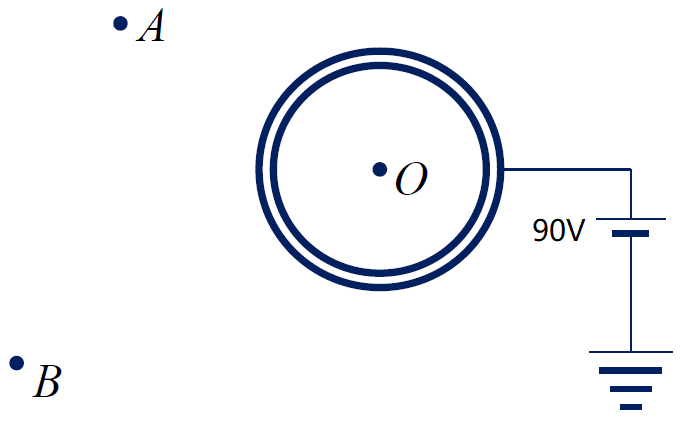
\includegraphics[width=3.5cm]{Images/m_of_image.png}
    \end{figure}
\end{frame}

\begin{frame}{Exercise 3}
    Two long, straight copper pipes, each of radius $R$, are held a distance $2d$ apart. One is at potential $V_0$, the other at $- V_0$. Find the potential everywhere.
    \begin{figure}[htbp]
        \centering
        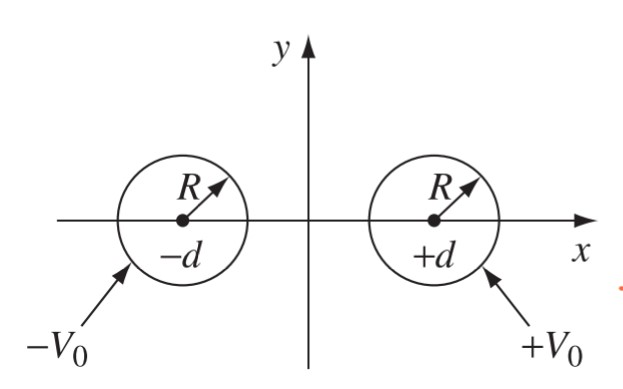
\includegraphics{Images/e3.jpg}
    \end{figure}
\end{frame}

\begin{frame}{Exercise 4}
    There exists a point charge $Q$ and a conducting shell in space. The distance between the center of shell 
    and the point charge is $a(a>R_0)$. Please find out the total amount of induced charge on the surface, in each case:
    \begin{itemize}
        \item The conducting shell is grounded
        \item The conducting shell is neither grounded nor carrying any charge at first
        \item The conducting shell is not grounded but at an electric potential $V_0$
        \item The conducting shell is not grounded but carrying charge $q$ at first
        \item What if $a<R_0$?
    \end{itemize}
\end{frame}

%----------------------------------------------------------------------------------------
%	 CLOSING/SUPPLEMENTARY SLIDES
%----------------------------------------------------------------------------------------

\begin{frame}
    \begin{center}
        \LARGE\bf Thanks for listening!
    \end{center}
	
\end{frame}


\section{Appendix}

%----------------------------------------------------------------------------------------

\begin{frame}{\bf References}
	\nocite{*} % Display all references regardless of if they were cited
	\bibliography{example.bib}
	\bibliographystyle{plain}
\end{frame}

\end{document}

